\documentclass[11pt,a4paper]{article}

% =========================================================
%  MECA-H419 — Data-Driven Engineering — Spring 2026
%  Project Group 5 — Predicting EU27 GHG Emissions
% =========================================================

\usepackage[utf8]{inputenc}
\usepackage[T1]{fontenc}
\usepackage{lmodern}
\usepackage[english]{babel}
\usepackage{amsmath,amssymb,amsthm}
\usepackage{graphicx}
\usepackage{booktabs}
\usepackage{geometry}
\geometry{margin=2.5cm}
\usepackage{hyperref}
\usepackage{caption}
\usepackage{subcaption}
\usepackage{siunitx}
\usepackage{cleveref}
\usepackage{xcolor}
\usepackage{placeins}
\usepackage[numbers]{natbib}

\hypersetup{colorlinks=true, linkcolor=black, citecolor=blue, urlcolor=blue}

% =========================================================
\title{Predicting EU27 Greenhouse-Gas Emissions\\
       from Sector-Level Data\\
       "Given the sector-level GHG emissions of EU27 countries in year t, predict the total EU27 emissions in year t+1"}
\author{{Group 5} \\[2pt]
        \small{MECA-H419 — Data-Driven Engineering, ULB}}
\date{June 2026}

\begin{document}
\maketitle

% =========================================================
\begin{abstract}
\noindent
% TODO — write last. ~150 words.
% (1) Problem: predict EU27 total GHG emissions at year t+1 from
%     sector-level emissions at year t.
% (2) Data: EDGAR 2025 booklet, 8 sectors, 4 substances, 55 years.
% (3) Methods: K-Means clustering + OLS / Ridge / Lasso regression,
%     validated on toy datasets (make_blobs, projectile).
% (4) Main results: ...
% (5) Take-away: ...
\end{abstract}

\tableofcontents
\newpage

% =========================================================
\section{Introduction and Methods}\label{sec:intro}

\subsection{Context and research question}\label{sec:context}
% TODO — briefly motivate the problem (climate policy, EU 2030/2050 targets,
% role of data-driven monitoring), then state the research question:
% "Given the sector-level GHG emissions of the EU27 in year t, predict
%  the total EU27 emissions in year t+1."

\subsection{Datasets}\label{sec:datasets}

\subsubsection{Toy datasets}
% TODO — describe make_blobs (synthetic clustering benchmark) and the
% projectile-motion analytical model used for regression validation.

\subsubsection{Real-world dataset}
% TODO — EDGAR 2025 GHG booklet \citep{edgar2025}: 194 countries,
% 8 sectors, 4 substances (CO2, CH4, N2O, F-gases, all in Mt CO2-eq via
% GWP-100 AR5), 55 annual records (1970--2024).

\subsection{Methods}\label{sec:methods}

\subsubsection{K-Means clustering}
% TODO — algorithm, Lloyd's iterations, objective function (inertia),
% elbow method / silhouette for choosing k, sensitivity to initialisation,
% limitations (spherical clusters, equal variance assumption).
% Key equation:
%   J = \sum_{i=1}^{k} \sum_{x \in C_i} \| x - \mu_i \|^2

\subsubsection{Linear regression: OLS, Ridge, Lasso}
% TODO — present the three estimators as a single regularised framework.
% Key equations to include:
%   OLS:   \hat\beta = \arg\min_\beta \| y - X\beta \|_2^2
%   Ridge: \hat\beta = \arg\min_\beta \| y - X\beta \|_2^2 + \lambda \|\beta\|_2^2
%   Lasso: \hat\beta = \arg\min_\beta \| y - X\beta \|_2^2 + \lambda \|\beta\|_1
% Discuss bias-variance trade-off, the role of \lambda, and how Lasso's
% L1 penalty yields sparsity (variable selection).

% =========================================================
\section{Toy Dataset Results}\label{sec:toy}

\subsection{Clustering validation on \texttt{make\_blobs}}
% TODO — show that K-Means recovers the known cluster structure;
% report ARI / accuracy vs. ground truth; show elbow plot.

\subsection{Regression validation on projectile motion}
% TODO — fit OLS/Ridge/Lasso to noisy projectile trajectories;
% compare to the analytical solution y = x \tan\theta - g x^2 / (2 v_0^2 \cos^2\theta);
% comment on coefficient recovery and the effect of \lambda.

% =========================================================
\section{Real Dataset Results}\label{sec:real}

\subsection{Data preparation}\label{sec:prep}

The raw EDGAR booklet contains $4{,}849$ rows, each row describing the annual
emissions (Mt~CO\textsubscript{2}-eq) of a (country, sector, substance) triplet
over the period 1970--2024. Before any modelling, the data are aggregated to
the EU27 level and transformed so that the eight sectoral features are
numerically comparable.

\subsubsection{Aggregation to EU27 sector level}\label{sec:prep-agg}

The EDGAR dataset already provides a pre-computed \texttt{EU27} entity (the
27~current EU member states aggregated according to the Union's official
composition), which we adopt to avoid re-implementing the aggregation
ourselves. For each of the four substances, we sum the contributions of the
eight emission sectors --- Agriculture, Buildings, Fuel Exploitation,
Industrial Combustion, Power Industry, Processes, Transport, Waste ---
yielding a clean matrix
\[
   E \in \mathbb{R}^{T \times S}, \qquad T = 55,\; S = 8,
\]
where $E_{t,s}$ is the total CO\textsubscript{2}-equivalent emission of
sector~$s$ in year~$t$. After aggregation, $E$ contains no missing values,
which is a key argument for working at the EU27 level rather than at the
country level (where several time series are incomplete, especially for the
pre-1990 period). The target variable is the annual total
\begin{equation}\label{eq:total}
   y_t \;=\; \sum_{s=1}^{S} E_{t,s} ,
\end{equation}
which drops from \SI{4572}{Mt\,CO_2\text{-}eq} in 1970 to
\SI{3165}{Mt\,CO_2\text{-}eq} in 2024 ($-30.8\%$, see
\Cref{fig:total-emissions}).

\begin{figure}[t]
   \centering
   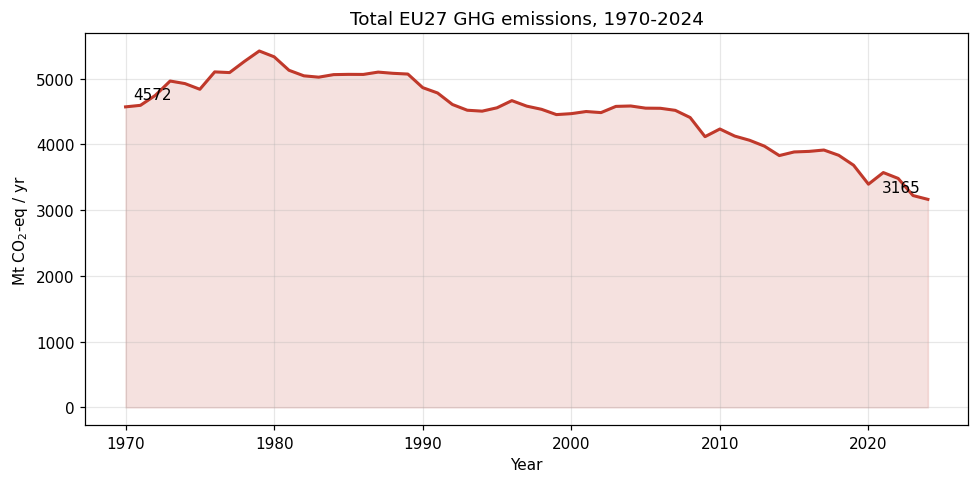
\includegraphics[width=0.85\linewidth]{figures/01_total_emissions.png}
   \caption{Total EU27 greenhouse-gas emissions, 1970--2024. Aggregated
            from EDGAR 2025 across the eight sectors and four substances.}
   \label{fig:total-emissions}
\end{figure}

\subsubsection{Log-transformation}\label{sec:prep-log}

Raw sectoral emissions span almost an order of magnitude --- the Power
Industry alone emits over \SI{1300}{Mt\,CO_2\text{-}eq/yr} in the
late~1980s, whereas Waste stays below \SI{200}{Mt\,CO_2\text{-}eq/yr} for the
entire period. Such heterogeneity makes a regularised regression unfair: the
penalty term $\lambda\|\beta\|$ would mechanically shrink the small-magnitude
features more aggressively. Because all entries of $E$ are strictly positive,
we apply a natural logarithm element-wise,
\begin{equation}\label{eq:log}
   \tilde{E}_{t,s} \;=\; \ln E_{t,s} ,
   \qquad
   \tilde{y}_t \;=\; \ln y_t ,
\end{equation}
which compresses the dynamic range from a factor of $\sim 7$ to a factor of
$\sim 1.5$ and stabilises the variance (\Cref{fig:dist-check}). It also
linearises any underlying exponential growth or decay, which makes the
resulting linear regression interpretable as a model of relative
(percentage) changes.

\begin{figure}[t]
   \centering
   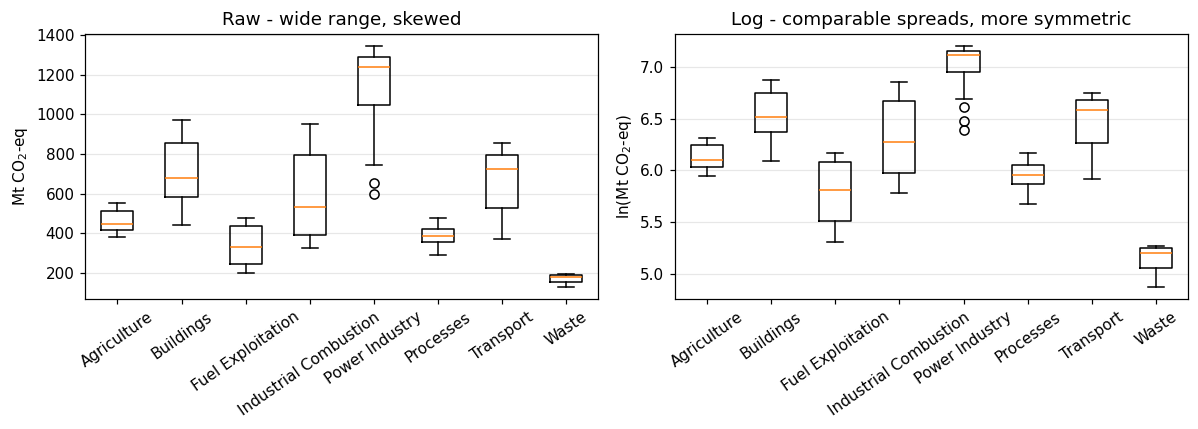
\includegraphics[width=0.95\linewidth]{figures/01_distribution_check.png}
   \caption{Distribution of sectoral emissions before (left) and after
            (right) the log-transformation. The log fixes the right-skew and
            brings sectors onto comparable spreads.}
   \label{fig:dist-check}
\end{figure}

\subsubsection{Standardization}\label{sec:prep-std}

After the log-transform, the eight features still have different means
($\overline{\tilde{E}_s}$ ranges from $\sim 5.1$ for Waste to $\sim 7.0$ for
Power Industry). To put them on the same scale, we apply a $z$-score
normalisation
\begin{equation}\label{eq:zscore}
   z_{t,s} \;=\; \frac{\tilde{E}_{t,s} - \mu_s}{\sigma_s},
   \qquad
   \mu_s = \frac{1}{T}\sum_t \tilde{E}_{t,s},
   \quad
   \sigma_s^2 = \frac{1}{T}\sum_t \bigl(\tilde{E}_{t,s} - \mu_s\bigr)^2 .
\end{equation}
After standardisation each feature has zero mean and unit variance, so
Ridge and Lasso penalties act symmetrically on every sector
(\Cref{fig:preprocessing}, right panel).

\textbf{A note on data leakage.} For the final modelling, $\mu_s$ and
$\sigma_s$ are recomputed from the \emph{training fold only} and then
applied unchanged to the validation/test folds; otherwise the test
statistics would influence the scaling. The global statistics shown in
\Cref{fig:preprocessing} are used only for exploratory visualisation.

\begin{figure}[t]
   \centering
   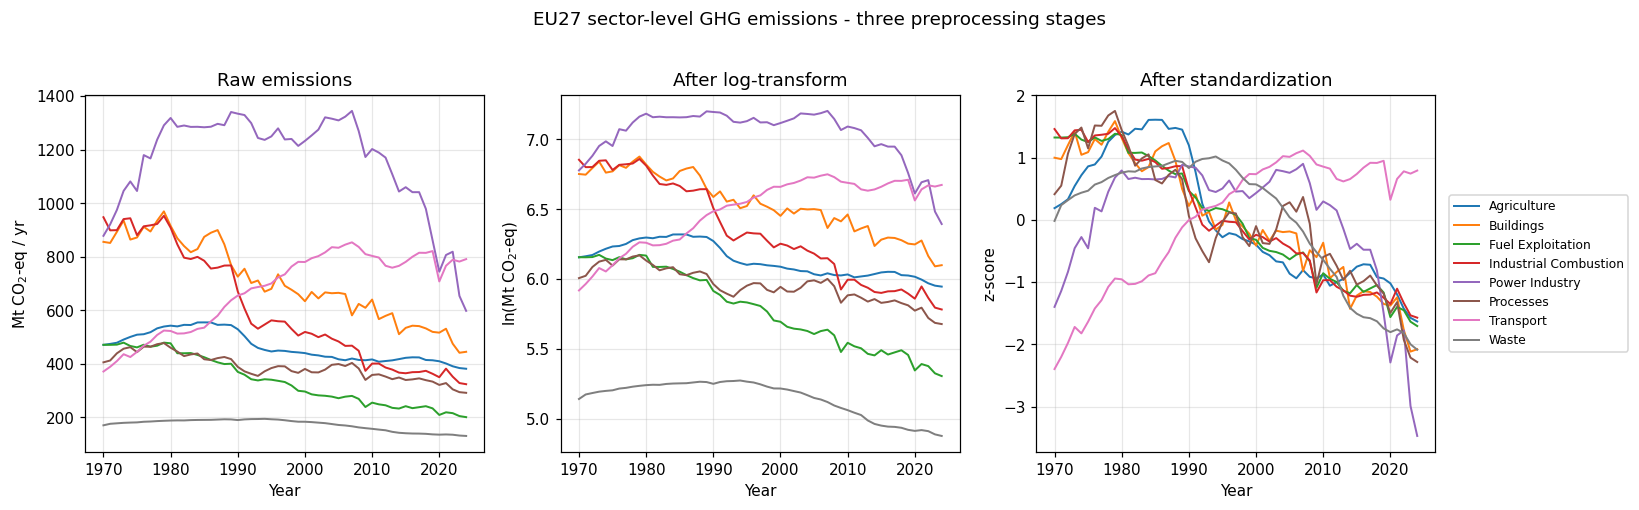
\includegraphics[width=\linewidth]{figures/01_preprocessing_stages.png}
   \caption{Sectoral EU27 emissions at the three stages of preprocessing:
            raw (left), after natural logarithm (centre), and after
            $z$-score standardisation (right). The transformations preserve
            the temporal patterns while equalising the numerical scale of
            the eight features.}
   \label{fig:preprocessing}
\end{figure}

\subsubsection{Supervised learning setup}\label{sec:prep-setup}

To address the research question
\emph{``given the sector-level emissions in year~$t$, predict the total
emissions in year~$t+1$''}, we build a one-step-ahead supervised dataset.
Each predictor row is a vector of the eight log-transformed sector
emissions, and the corresponding target is the next-year log-total:
\begin{equation}\label{eq:supervised}
   \mathbf{x}_t \;=\; \bigl(\tilde{E}_{t,1},\,\ldots,\,\tilde{E}_{t,S}\bigr) \in \mathbb{R}^{8},
   \qquad
   y_t' \;=\; \tilde{y}_{t+1} \in \mathbb{R} ,
   \qquad
   t = 1970, \ldots, 2023.
\end{equation}
This yields $N = 54$ paired observations
$\{(\mathbf{x}_t, y_t')\}_{t=1970}^{2023}$, with predictors covering
1970--2023 and targets covering 1971--2024.
\Cref{tab:prep-summary} summarises the pipeline.

\begin{table}[h]
\centering
\caption{Summary of the preprocessing pipeline for the real-world dataset.}
\label{tab:prep-summary}
\begin{tabular}{lll}
\toprule
\textbf{Stage}      & \textbf{Operation}                                & \textbf{Resulting shape} \\
\midrule
Raw EDGAR booklet   & Filter \texttt{EU27}, $4{\times}8 - 7$ rows        & $25 \times 55$           \\
Aggregation         & Sum substances per sector (\Cref{eq:total})        & $E \in \mathbb{R}^{55\times 8}$ \\
Log-transform       & Natural log of $E$ and total (\Cref{eq:log})       & $\tilde{E},\,\tilde{y}$  \\
Standardization     & $z$-score on training fold (\Cref{eq:zscore})      & $z,\,\tilde{y}_\text{std}$ \\
Supervised pairs    & $(\mathbf{x}_t, y_t') = (\tilde{E}_t, \tilde{y}_{t+1})$ \, (\Cref{eq:supervised}) & $N = 54$ \\
\bottomrule
\end{tabular}
\end{table}

\subsection{Clustering of countries}\label{sec:clustering}

The main objective of this project is to predict the total greenhouse gas emissions of the EU27. However, the aggregated EU dataset only provides 54 years of historical data ($N=54$). Training a regression model on such a small dataset can be difficult and may lead to overfitting or poor predictions. To solve this problem, an unsupervised learning step was introduced before the main regression task. The goal of this clustering step is to analyze the 194 global countries and group them by their industrial and economic profiles. By identifying which countries around the world share the same emission patterns as the European member states, the training dataset can potentially be expanded with similar global countries to build a stronger and more accurate prediction model.

\subsubsection{Data Preparation for Clustering}
Before grouping the 194 countries from the EDGAR dataset, the data had to be prepared differently than for the regression. The goal was to group countries by what their economy looks like today, not by how big they are or their past emissions. So, only recent years were used.

First, big groups like ``EU27'', ``GLOBAL TOTAL'', and international transport zones were removed. Then, all the emissions for each sector were added up and the average for the last 15 years (2010--2024) was calculated. 

To make sure the computer looks at the shape of the emissions and not the total size of the country, the numbers were changed into percentages (like Sector Emissions / Total Country Emissions). Finally, a z-score standardization (StandardScaler) was applied. This was done because some sectors (like Waste) are small and do not change much. It was important to make sure these small sectors were just as important for the K-Means as big sectors like the Power Industry.

\subsubsection{K-Means Optimization and Silhouette Analysis}
After the data was ready, K-Means was used to find groups of countries with similar emissions. To find the best number of groups ($K$), the Silhouette Score was checked for $K$ from 2 to 10. 

The best score was $0.2453$ when $K=8$. A score of about $0.25$ means some groups overlap a little bit, but it still shows a real difference between the country profiles. So, $K=8$ was chosen for the final model.

\begin{figure}[htbp]
    \centering
    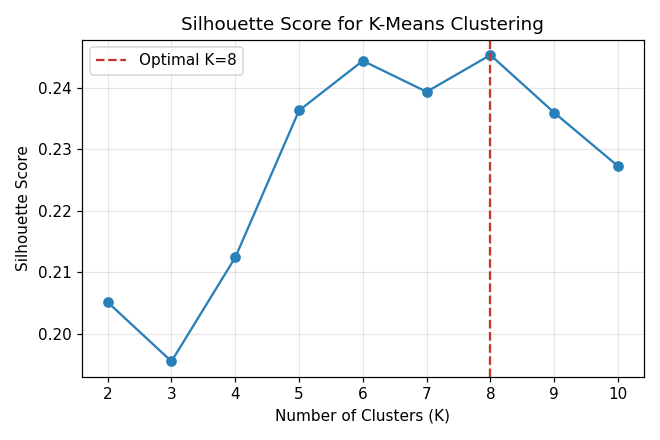
\includegraphics[width=0.72\linewidth,height=0.34\textheight,keepaspectratio]{figures/02_silhouette_scores.png}
    \caption{Silhouette scores for different numbers of clusters ($K$). The peak at $K=8$ indicates the optimal mathematical separation of global emission profiles.}
    \label{fig:silhouette}
\end{figure}

\subsubsection{The Fragmentation of the EU27}
A very important result from this step is that the EU27 countries are not all in the same group. At first, it seemed like the EU would have one single profile. But the countries have very different economies, so the EU27 is actually split into three different groups.

\begin{figure}[htbp]
    \centering
    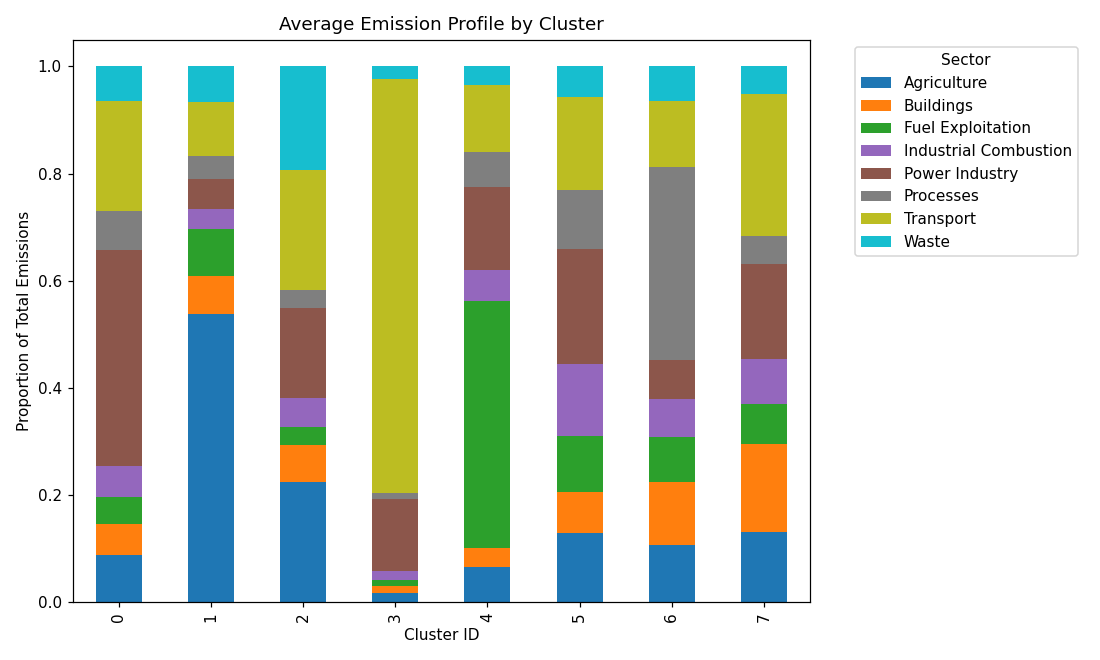
\includegraphics[width=0.92\linewidth,height=0.48\textheight,keepaspectratio]{figures/02_cluster_profiles.png}
    \caption{Average sectoral emission profiles for the three clusters containing EU27 member states. Values represent the percentage contribution of each sector to the country's total emissions.}
    \label{fig:cluster-profiles}
\end{figure}
\FloatBarrier

The 27 countries are in Cluster 0 (7 countries), Cluster 5 (10 countries), and Cluster 7 (10 countries). Here is what these groups look like:

\begin{itemize}
    \item \textbf{Cluster 0 (High Power Industry):}
    \begin{itemize}
        \item \textit{Members (7):} Bulgaria, Cyprus, Czechia, Estonia, Greece, Malta, Poland.
        \item \textit{Profile:} These countries have a lot of emissions from the Power Industry (about 40.3\% on average). This means they probably still use a lot of coal and fossil fuels for their electricity.
    \end{itemize}
    
    \item \textbf{Cluster 5 (Balanced Industry):}
    \begin{itemize}
        \item \textit{Members (10):} Austria, Croatia, Finland, Lithuania, Portugal, Romania, Slovakia, Slovenia, Spain, Sweden.
        \item \textit{Profile:} This group is very balanced. They have Power Industry emissions (21.5\%), but also higher emissions from Industrial Combustion (13.4\%) and Agriculture (13.0\%) than the other European countries.
    \end{itemize}
    
    \item \textbf{Cluster 7 (Transport and Buildings):}
    \begin{itemize}
        \item \textit{Members (10):} Belgium, Denmark, France, Germany, Hungary, Ireland, Italy, Latvia, Luxembourg, Netherlands.
        \item \textit{Profile:} Most of their emissions come from Transport (26.6\%) and Buildings (16.5\%). Their Power Industry is lower (17.9\%). This is normal for rich countries that have cleaner electricity but lots of cars and need a lot of heating for houses.
    \end{itemize}
\end{itemize}

\subsubsection{Implications for Supervised Modelling}
Because there is no single ``EU27 group,'' there is a problem for the next step (the regression). The total EU emissions are actually a mix of three very different types of economies. So, the model cannot just be trained on one ``global EU'' group anymore. 

For the supervised step, the plan has to change. Either (a) three different models must be made for the three groups and the results added together, or (b) a new training dataset must be created that mixes the three groups in the same 7:10:10 ratio to predict the total EU27 emissions.

\subsection{Predicting EU27 emissions}\label{sec:regression}
% TODO — Step 3: train OLS / Ridge / Lasso on (a) all countries pooled
% and (b) EU27 cluster only; cross-validation strategy
% (TimeSeriesSplit), regularisation-path plots, coefficient
% interpretation, residual diagnostics.

\subsection{Forecast 2025--2034}\label{sec:forecast}
% TODO — Step 4: iterative one-step-ahead forecast, propagation of
% uncertainty (e.g. block bootstrap), comparison with EU's official
% projections.

% =========================================================
\section{Discussion and Conclusions}\label{sec:conclusion}
% TODO — when does each model dominate? what are the limitations
% (no climate-policy variables, no shocks)? what would the natural
% extensions be (non-linear methods, neural networks --- bonus)?

% =========================================================
\section*{AI Disclosure}
We use Claude, ChatGPT, GitHub Copilot, etc for these tasks ...

% =========================================================
\bibliographystyle{plainnat}
\begin{thebibliography}{9}

\bibitem{edgar2025}
European Commission, Joint Research Centre (JRC).
\newblock \emph{EDGAR -- Emissions Database for Global Atmospheric Research, GHG Booklet 2025}.
\newblock 2025.

\bibitem{esl}
T.~Hastie, R.~Tibshirani, J.~Friedman.
\newblock \emph{The Elements of Statistical Learning}.
\newblock Springer, 2nd ed., 2009.

\bibitem{sklearn}
F.~Pedregosa et~al.
\newblock Scikit-learn: Machine Learning in Python.
\newblock \emph{J. Machine Learning Res.}, 12:2825--2830, 2011.

\end{thebibliography}

% =========================================================
\appendix
\section{Appendix}\label{sec:appendix}
% TODO — supplementary tables/figures, derivations, additional sensitivity
% analyses. A reproducibility note pointing to the code repository goes here.

\end{document}